\documentclass[10pt,leqno]{report}
\usepackage{amsmath,amssymb,graphicx,enumitem} 
\usepackage{calc}
\usepackage[T1]{fontenc}
\usepackage{tcolorbox,parskip}
\usepackage{float}
\floatstyle{boxed}
\restylefloat{figure}
\graphicspath{{/Users/econhead/NOTES/Microeconomics/MicroClassNotes/Figures/}}
\usepackage{fancyhdr}
\setlength{\headheight}{14pt}
\pagestyle{fancyplain}
\fancyhead[L]{Laxman Singh}
\fancyhead[R]{October 5th, 2024}
\begin{document}
\section*{1. Extensive Games with Perfect Information}
An Extensive game with perfect information consists of the following ; 
\begin{itemize}
    \item Set of players 
    \item Set of Sequences (terminal histories) with proper entry that no sequence is a proper subhistory of any other sequence. 
    \item A player function that assigns a player to every sequence that is a proper subhistory of some terminal history. 
    \item Prefernces for each player over the set of terminal histories. 
\end{itemize}
\subsection*{Examples}
\textbf{\underline{Game 1:}} \textit{Simultaneous move Duoploy}
\begin{tcolorbox}
An enterant firm decides to enter an Industry or not while the icumbent firm in that industry decides to wether to accomodate or fight the new enterant firm.\\
\begin{itemize}
\item Set of players: \\ \(N={\mathrm{Enterant(E),Incumbent(I)}}\) \\
\item Action Set of Each Player: \\ \(T=\{\mathrm{Stay Out,(Enter,Fight),(Enter,Acommodate)}\}\) \\
\item Player Function: \\ \(\mathcal{P}(\phi)=\text{E}\) \\ 
      \(\mathcal{P}(\text{Enter})= \text{I}\)\\
\item Payoffs of both players: \\ \(U_{E}(\text{Stay out})=0\)\\
      \(U_{E}(\text{Enter,Fight})=-50\)\\
      \(U_{E}(\text{Enter,Accomodate})=50\)\\
      \(U_{I}(\text{Stay out})=100\)\\
      \(U_{I}(\text{Stay out})=0\)\\
      \(U_{I}(\text{Stay out})=50\)\\
\end{itemize}
\end{tcolorbox}
\begin{figure}[H]
    \centering
     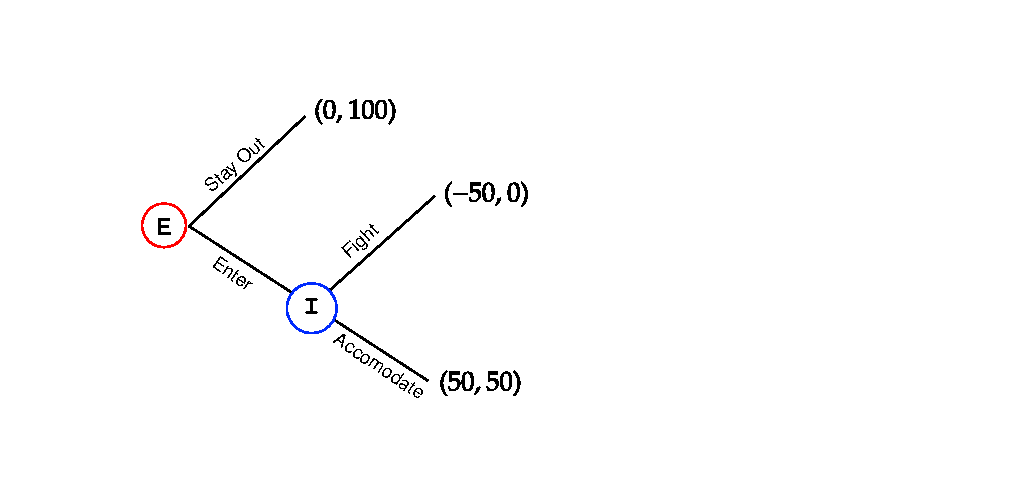
\includegraphics[scale=0.6]{gametree.pdf}
    \caption{Simultaneous move Duopoly}
\end{figure}
Nash Equilibrium, \ \(NE=\{\mathrm{(Stay out,Fight),(Enter,Accomodate)}\}\) \\
Subgame Perfect Equilibrium, \ \(SPE=\{\mathrm{(Enter,Accomodate)}\}\)\\
\linebreak
Note that \(\mathrm{(Stay out, Fight)}\) is a Nash equilbrium but not a subgame perfect equilibrium because it is not a Nash Equilibrium of every subgame in this game. \\

\textbf{\underline{Game 2:}} @3866, \textit{Piazza Contributing Efforts game}

\begin{tcolorbox}
    Consider the following simultaneous-move effort-contributions' game of $n$ players: 
    \begin{itemize}
        \item Set of players: $\{1,2,\ldots,n\}$
        \item Action set of each player : $A_i=[0,1]$
        \item Payoff of player : $u_i(e_1,e_2,\ldots, e_n)=n\min(e_1,e_2,\ldots,e_n)-e_i$
    \end{itemize} 
    \vspace{2pt}
    Let us solve this game for $n=3$ players; \\ 
    \begin{itemize}
        \item Strategy of player 3: \(S_{3}: [0,1] \times [0,1] , \ \ S_{3}(e_{1},e_{2})\)
        \item Strategy of Player 2: \(S_{2}: \ \ S_{2}(e_{1})\)
        \item Strategy of Player 1: \(S_{1} \in [0,1]\)
    \end{itemize} 
 \end{tcolorbox}   
 \begin{figure}[H]
    \centering
     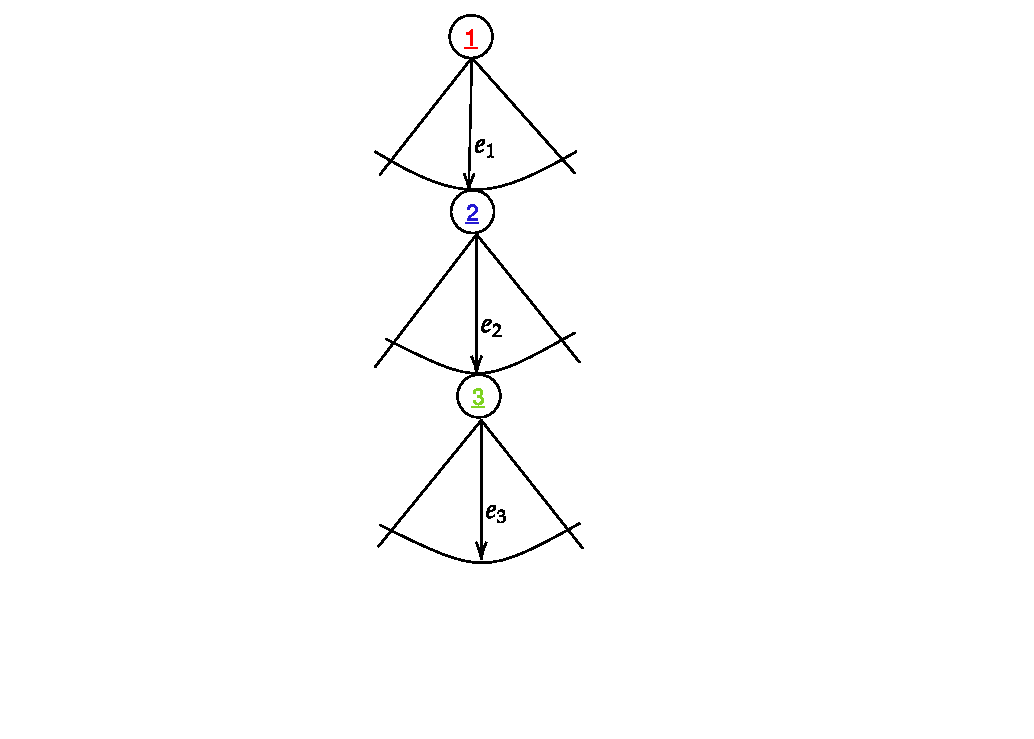
\includegraphics[scale=0.5]{gametree2.pdf}
    \caption{Efforts Contribution Game}
\end{figure}  
    Solving the game using backward induction, We solve for the player $3$ first; \\
    Player 3 will solve the following utility maximization problem given $(e_{1},e_{2})$;
    \begin{equation*}
        \max_{0\leq e_{3} \leq 1}  3\min(e_{1},e_{2},e_{3})-e_{3}
    \end{equation*}
    \begin{figure}[H]
        \centering
         \includegraphics[scale=0.6]{game2_1.pdf}
        \caption{Payoff function of player 3 }
    \end{figure}   
    The solution to this problem is; \(e_{3}=S_{3}(e_{1},e_{2})=\min(e_{1},e_{2})\)\\
    Folding the game backward again, Player 2 will now solve his following utility maximization problem given \(e_{1}\);
    \begin{eqnarray*}
        \max_{0\leq e_{2} \leq 1} & 3\min(e_{1},e_{2},e_{3})-e_{2} \\
        s.t. & e_{3}=S_{3}(e_{1},e_{2})=\min(e_{1},e_{2}) 
    \end{eqnarray*}
    \begin{figure}[H]
        \centering
         \includegraphics[scale=0.6]{game2_2.pdf}
        \caption{Payoff function of player 2 }
    \end{figure}
    Solving the above problem by substituting for \(e_{3}\) into the objective function we can rewrite our problem as 
    \begin{equation*}
        \max_{e_{1},e_{2}} 3\min(e_{1},e_{2})-e_{2}
    \end{equation*}
    solving this we get, \(e_{2}=S_{2}(e_{1})=e_{1}\)\\
    And then finally player 1 solves his utilty maximization problem;
    \begin{eqnarray*}
        \max_{0\leq e_{1} \leq 1} & 3\min(e_{1},e_{2},e_{3})-e_{1}\\
        s.t. & e_{3}=S_{3}(e_{1},e_{2})=\min(e_{1},e_{2})\\
        & e_{2}=e_{1}
    \end{eqnarray*}
    Solving the above gives \(e_{1}=1\)\\
    Therefore \(e_{1}^*=e_{2}^*=e_{3}^*=\min(e_{1},e_{2})=1\)\\
    And the resulting terminal History where players move according to the equilibrium strategy \((1,1,1)\) is the Subgame Perfect Equilibrium outcome and the SPE stratrgy is; \\
    \begin{align*}
        e_{1}&=S_{1}=1\\
        e_{2}&=S_{2}=e_{1}\\
        e_{2}&=S_{3}(e_{1},e_{2})=\min(e_{1},e_{2})
    \end{align*}
\linebreak    
\textbf{\underline{Game 3:}} \textit{Stackelberg Duopoly Using Isoprofit Curves}
\begin{tcolorbox}
\begin{enumerate}
\item Set of Players; \\
\(N=\{1,2\}\)
\item Action set of players; \\
\(T=\{(q_{1},q_{2})\in \mathbb{R}_{+} \times \mathbb{R}_{+}\}\)
\item Player function;
 \begin{flalign*}
&\mathcal{P}(\phi)=1&\\
&\mathcal{P}(q_{1})=2, \forall q_{1}\in \mathbb{R}_{+}&
 \end{flalign*}
\item Payoff of palyer $i \ \  \forall \ i\in\{1,2\}$; \\
\(\pi_{i}(q_{1},q_{2})=q_{i}\max(15-q_{1}-q_{2},0)\)
\end{enumerate}
\end{tcolorbox}
Solving this game Using Backward Induction;\\
First firm 2(follower) solves its profit maximization problem taking output of firm 1, \(q_{1}\) as given; 
\begin{eqnarray*}
    \max_{q_{2}\geq 0} q_{2}(\max(15-q_{1}-q_{1},0))
\end{eqnarray*}
    Solution to which gives us the best response function of player 2 given  \(q_{1}, \ BR_{2}(q_{1})\)
\begin{eqnarray*}
    BR_{2}(q_{1})\in \begin{cases}
        \{\frac{15-q_{1}}{2}\} &  \text{if} \ \ q_{1} < 15\ \\
        \mathbb{R}_{+}  & \text{if} \ \ q_{1}\geq 15
    \end{cases}
\end{eqnarray*}
So, 
\begin{eqnarray*}
    q_{2}(q_{1})=\begin{cases}
        \frac{15-q_{1}}{2} &  \text{if} \ \ q_{1} < 15\ \\
        0  & \text{if} \ \ q_{1}\geq 15
    \end{cases}
\end{eqnarray*}
Then the firm 1(leader) solve its profit maximization problem subject to the best response fucntion of the follower;
\begin{eqnarray*}
    \max_{q_{1}\geq 0} & q_{1}(\max(15-q_{1}-q_{2},0))\\
    s.t. & q_{2}(q_{1})=\begin{cases}
        \frac{15-q_{1}}{2} &  \text{if} \ \ q_{1} < 15\ \\
        0  & \text{if} \ \ q_{1}\geq 15
    \end{cases} 
\end{eqnarray*}
The above problem can be rewritten as;
\begin{eqnarray*}
    \max_{0\leq q_{1} \leq 15} q_{1} \big(\frac{15-q_{1}}{2}\big)
\end{eqnarray*}
solving which gives us the following;
 \(q_{1}^*=7.5,q_{2}^*=\frac{7.5}{2}\) \\
\linebreak
The above problem can also be solved using the isoprofit curves approach as follow; \\
\begin{flalign*}
& q_{1}(15-q_{1}-q_{2})=\overline{\pi}&\\
& \text{differntiating both sides w.r.t} \ q_{1}&\\
& \implies \dfrac{\mathrm{d}q_{1}}{\mathrm{d}q_{2}} = \frac{15-2q_{1}-q_{2}}{q_{1}}&\\
& \text{But,}  \ \ \dfrac{\mathrm{d}q_{2}}{\mathrm{d}q_{1}}=\frac{-1}{2}&\\
&\implies \frac{15-2q_{1}-q_{2}}{q_{1}}=\frac{-1}{2}&\\
&\implies q_{1} = 7.5, q_{2}=3.75
\end{flalign*} 
\begin{figure}[H]
    \centering
     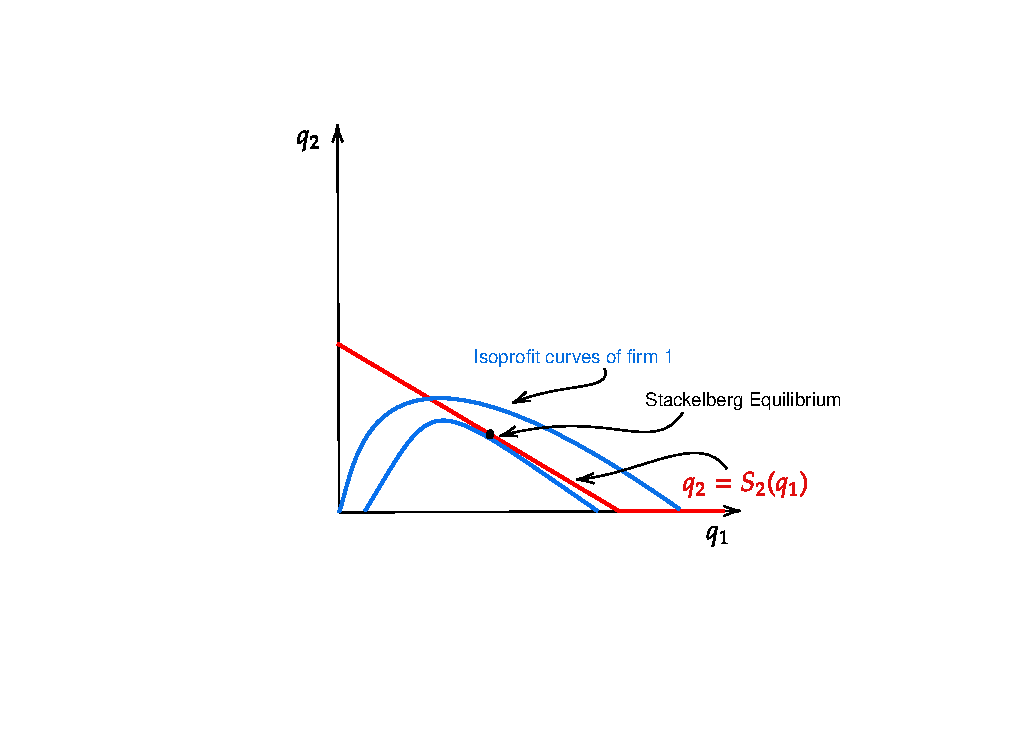
\includegraphics[scale=0.6]{Game3.pdf}
    \caption{Stackelberg Equilibrium }
\end{figure} 
\pagebreak
\textbf{\underline{Game 4:}} \textit{Stackelberg Duopoly with fixed costs} \\
\begin{tcolorbox}
    \begin{itemize}
        \item \(\pi_{i}=q_{i}\max(16-q_{1}-q_{2},)-F_{i}\ ; \ \text{if} \ q_{i}>0\)
        \item \(F_{i}(q_{i})=\begin{cases}
            25 & \text{if} \ q_{i}>0 \\
            0 & \text{if} \ q_{i}=0
        \end{cases}\)
    \end{itemize}
\end{tcolorbox}
Solving using backward induction follower firm 2 solves its profit maximization problem first taking \(q_{1}\) as given;\\
\begin{align*}
    \max_{q_{2}>0} \ q_{2}(\max(16-q_{1}-q_{2},0))-25 
\end{align*}
Solving which gives us, \\
\begin{eqnarray*}
    BR_{2}(q_{1})\in \begin{cases}
        \{\frac{16-q_{1}}{2}\} &  \text{if} \ \ q_{1} < 6\ \\
        \mathbb{R}_{+}  & \text{if} \ \ q_{1}\geq 6
    \end{cases}
\end{eqnarray*}
and, 
\begin{eqnarray*}
    q_{2}(q_{1})=\begin{cases}
        \frac{16-q_{1}}{2} &  \text{if} \ \ q_{1} < 6\ \\
        0  & \text{if} \ \ q_{1}\geq 6
    \end{cases}
\end{eqnarray*}
Then the leader firm 1 solves it's profit maximization problem subject to followers's best response;
\begin{eqnarray*}
    \max_{q_{1}\geq 0} & q_{1}(\max(16-q_{1}-q_{2},0))-25 \\
    s.t. & q_{2}(q_{1})=\begin{cases}
        \frac{16-q_{1}}{2} &  \text{if} \ \ q_{1} < 6 \\
        0  & \text{if} \ \ q_{1}\geq 6
    \end{cases} 
\end{eqnarray*}
The solution to this problem is that firm 1 will produce the monoply outcome of \(q_{1}=8\) given follower's strategy and \(q_{2}=0\). This game is also known as Natural Monopoly since the monopoly output is enough to deter the entry of the follower firm. 
\linebreak

\textbf{\underline{Game 5:}} \textit{Stackelberg Duopoly with fixed costs} \\
\begin{tcolorbox}
    \begin{itemize}
        \item \(\pi_{i}=q_{i}\max(16-q_{1}-q_{2})-F_{i}\ ; \ \text{if} \ q_{i}>0\)
        \item \(F_{i}(q_{i})=\begin{cases}
            9 & \text{if} \ q_{i}>0 \\
            0 & \text{if} \ q_{i}=0
        \end{cases}\)
    \end{itemize}
\end{tcolorbox}
Solving using backward induction follower firm 2 solves its profit maximization problem first taking \(q_{1}\) as given;\\
\begin{align*}
    \max_{q_{2}>0} \ q_{2}(\max(16-q_{1}-q_{2},0))-9 
\end{align*}
Solving which gives us, \\
\begin{eqnarray*}
    BR_{2}(q_{1})\in \begin{cases}
        \{\frac{16-q_{1}}{2}\} &  \text{if} \ \ q_{1} < 10\ \\
        \mathbb{R}_{+}  & \text{if} \ \ q_{1}\geq 10
    \end{cases}
\end{eqnarray*}
and, 
\begin{eqnarray*}
    q_{2}(q_{1})=\begin{cases}
        \frac{16-q_{1}}{2} &  \text{if} \ \ q_{1} < 10\ \\
        0  & \text{if} \ \ q_{1}\geq 10
    \end{cases}
\end{eqnarray*}
Then the leader firm 1 solves it's profit maximization problem subject to followers's best response;
\begin{eqnarray*}
    \max_{q_{1}\geq 0} & q_{1}(\max(16-q_{1}-q_{2},0))-9 \\
    s.t. & q_{2}(q_{1})=\begin{cases}
        \frac{16-q_{1}}{2} &  \text{if} \ \ q_{1} < 10 \\
        0  & \text{if} \ \ q_{1}\geq 10
    \end{cases} 
\end{eqnarray*}
Unlike the previous game the monopoly outcome \(q_{1}=8\) is not enough to deter the entry and hence the leader firm produces \(q_{1}=10\) now and \(q_{2}=0\). This case is known as the Entry deterrence case.

\textbf{\underline{Game 6:}} \textit{Stackelberg Duopoly with fixed costs} \\
\begin{tcolorbox}
    \begin{itemize}
        \item \(\pi_{i}=q_{i}\max(16-q_{1}-q_{2})-F_{i}\ ; \ \text{if} \ q_{i}>0\)
        \item \(F_{i}(q_{i})=\begin{cases}
            1 & \text{if} \ q_{i}>0 \\
            0 & \text{if} \ q_{i}=0
        \end{cases}\)
    \end{itemize}
\end{tcolorbox}
Solving using backward induction follower firm 2 solves its profit maximization problem first taking \(q_{1}\) as given;\\
\begin{align*}
    \max_{q_{2}>0} \ q_{2}(\max(16-q_{1}-q_{2},0))-1 
\end{align*}
Solving which gives us, \\
\begin{eqnarray*}
    BR_{2}(q_{1})\in \begin{cases}
        \{\frac{16-q_{1}}{2}\} &  \text{if} \ \ q_{1} < 14\ \\
        \mathbb{R}_{+}  & \text{if} \ \ q_{1}\geq 14
    \end{cases}
\end{eqnarray*}
and, 
\begin{eqnarray*}
    q_{2}(q_{1})=\begin{cases}
        \frac{16-q_{1}}{2} &  \text{if} \ \ q_{1} < 14\ \\
        0  & \text{if} \ \ q_{1}\geq 14
    \end{cases}
\end{eqnarray*}
Then the leader firm 1 solves it's profit maximization problem subject to followers's best response;
\begin{eqnarray*}
    \max_{q_{1}\geq 0} & q_{1}(\max(16-q_{1}-q_{2},0))-1 \\
    s.t. & q_{2}(q_{1})=\begin{cases}
        \frac{16-q_{1}}{2} &  \text{if} \ \ q_{1} < 14 \\
        0  & \text{if} \ \ q_{1}\geq 14
    \end{cases} 
\end{eqnarray*}
In this case the fixed costs are so low that leader firm decides to accomodate the entry and produces \(q_{1}=8\) and the follower produces \(q_{2}=8\). 

\end{document}
